Finite elements of class $C^1$ are of particular interest when employing
conforming finite elements for partial differential equations of order four, such
as the Biharmonic equation. If we are to require conformal finite elements,
Lagrange finite elements are not enough to guarantee continuity in the first
derivative, and so to ensure continuity in the first derivative the Argyris
Element (depicted in Figure \ref{fig:Argyris}) or Bell's Element should
be used \cite{Johnson}. The Argyris element is probably the best known of all
$C^1$ finite elements \cite{Argyris,DominguezA}, but appear to be rarely
implemented.

\begin{figure}[h]
	\begin{center}
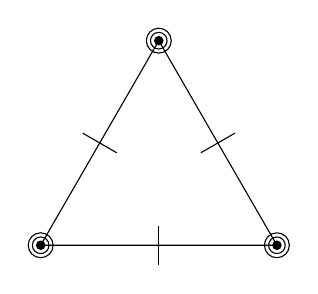
\begin{tikzpicture}[scale=0.5]
	%define the vertices of the triangle
	\path[coordinate] (0,0) coordinate(A)
		++(60:3cm) coordinate(D)
		++(60:3cm) coordinate(B)
		++(-60:3cm) coordinate(E)
		++(-60:3cm) coordinate(C)
		++(180:3cm) coordinate(F);
	%label the vertices and draw edges
	\draw (A) -- (D) -- (B) -- (E) -- (C) -- (F) -- cycle;
	%draw the interpolation points
	%function values
	\filldraw[black] (A) circle(3pt); 
	\filldraw[black] (B) circle(3pt); 
	\filldraw[black] (C) circle(3pt); 
	%first derivatives
	\draw[black] (A) circle(6pt); 
	\draw[black] (B) circle(6pt); 
	\draw[black] (C) circle(6pt); 
	%second derivatives
	\draw[black] (A) circle(9pt); 
	\draw[black] (B) circle(9pt); 
	\draw[black] (C) circle(9pt); 
	%normal derivatives
	\draw (1.067,2.848) -- (D) -- (1.933,2.348); 
	\draw (4.067,2.348) -- (E) -- (4.933,2.848); 
	\draw (3,-0.5cm) -- (F) -- (3,0.5cm); 
	%labels
%	\node[below of=A, node distance=0.5cm] (k) {$k=j+1$};
% \node[above of=B, node distance=0.5cm] (j) {$j=i+1$};
%	\node[below of=C, node distance=0.5cm] (i) {$i$};
\end{tikzpicture}
	\end{center}
	\caption{Argyris element with its 21 degrees of freedom.}
	\label{fig:Argyris}
\end{figure}


The Argyris element does, in fact, ensure $C^1$ continuity
\cite{DominguezA,Okabe}, but at a cost of twenty-one degrees of freedom.
However, these twenty-one degrees of freedom give basis polynomials of degree
five and therefore has a very high rate of convergence \cite{DominguezA}. These
degrees of freedom include the value at each vertex, the value of the first
derivatives at each vertex, the value of the second derivatives at each vertex,
the value of the mixed derivative at each vertex, and finally the value of the
normal derivatives at each of the edge midpoints. Here in lies the main
difficulty in implementing the Argyris triangle, the normal derivatives. Not
only do we now have 21 degrees of freedom that we must worry about, but the
added complexity of a transformation that maintains the direction of the normal
derivations is required. Since working on the reference element is the most
common way of working finite elements and normal derivatives are not respected
by affine transformation a more complicated transformation will have to be
employed \cite{DominguezA}. This is unlike a standard Lagrange element where
only require a simple Affine transformation, since directional derivative are
not considered.

In what follows a ``simple'' implementation of the Argyris finite element will
be discussed. The transformation that was developed by Dominguez \emph{et. al.}
will allow for all calculations to be done on a reference element, vastly
simplifying the calculations of the mass matrix, stiffness matrix, bending
matrix and load vector. In addition to a discussion of the Argyris finite
element a brief description of a method to allow for basis function calculations
to be performed as dot products or matrix-vector multiplication will be
discussed.

Finally, the code will be checked by applying it to a test problem. The test
problem that I will consider is the Biharmonic equation in two-dimensions. The
Biharmonic equation is a fourth-order partial differential equation and
therefore a good problem for testing the Argyris finite elements. In this
problem the $L^2,\; H^2,\text{ and } L^{\infty}$ error will be computed so as to
observe the rate of convergence.
